\cotefile{79}
\scanpage{175}
% L01–02
On a commutativité dans

\diagram{\begin{tikzcd}[ampersand replacement=\&,column sep=large]
Z \arrow[r,"{\unsure{\varphi_Z|\psi_Z|\varphi Z}}","{(53)}"'] \arrow[dr,"{(50\,b)}"'] \& G \arrow[d,"{\deleted{\unsure{a}}(52'\,a)}"]\\
\& Z'.
\end{tikzcd}}

% L03–05
Nous allons expliciter maintenant les particularités des données (54), dans le cas qui nous occupe.

% L06–07
\noindent\makebox[0pt][r]{(56)\quad}1) Le groupe $G_0$ a des générateurs $\tau_0,\tau_1,\tau_\infty$ satisfaisant les conditions (21)

% L08–09
2) $\widetilde U={}$sous-groupe engendré par $\tau_1,\tau_\infty$, isomorphe à $D_n$ (non canoniquement)

% L10–13
3) Opération fidèle de $G$ sur $S$, ce qui s'exprime par la fidélité de l'opération de $B'\inserted{(\simeq G_{s_0})}$ sur $S\simeq G_0/\widetilde U$, opération déduite de l'opération de $B'$ sur $G_0$, stabilisant $U_0$ et passant donc au quotient
\margin{donc $B'$ opère fidèlement sur $G_0$, et peut donc s'interpréter comme un \uline{sous-groupe} de $\operatorname{Aut}_{\mathrm{gr}}(G_0\supset\widetilde B''\supset\widetilde U)$ contenant l'image de $\widetilde B''$ dans ce groupe d'automorphismes (ce qui explicite en $=$ temps $\psi:\widetilde B''\to B'$}

% L14–19
4) $Z'=Z$ et $Z\longrightarrow Z'=Z$ est l'hom $\lambda\mapsto\lambda^2$, en d'autres termes la donnée b) de (50), est une façon d'exprimer l'extension $\widetilde B''$ de $Z$ par $\widetilde U$ comme déduite d'une \uline{autre} extension $\inserted{B'}$ de $=$ $Z$ par $\widetilde U$, \inserted{(par image inv.)} via l'hom $Z\longrightarrow Z^2$ (``carré'' \unsure{d'une|d'un|de} \unsure{autre|côté|l'ext.} $B'$).

% L20
Donc on peut expliciter les données \unsure{admise|arrivée|ainsi :|ainsi}

% archive sheet number: 174
\scanpage{176}
\mspage{90}
% L01–02
\noindent\makebox[0pt][r]{\smash{\raisebox{-15\baselineskip}{$(57)\ \left\{\rule{0pt}{30\baselineskip}\right.$}}\quad}a) Un groupe quotient $G_0$ du groupe cartographique triangulé $\unsure{\mathcal C_{\infty,3}|G_{\infty,3}|\mathfrak C_{\infty,3}}\simeq\{\tau_0,\tau_1,\tau_\infty\mid\tau_0^2=\tau_1^2=\tau_\infty^{2}=(\underbrace{\tau_1\tau_\infty}_{\rho_\infty})^3=(\underbrace{\tau_0\tau_\infty}_{\rho_1})^2=\}$

% L03–06
b) Un sous-groupe $\widetilde B''$ \deleted{\unsure{disons|du normalisateur}} \inserted{de $G_0$,} contenant le sous-groupe $\widetilde U$ engendré par $\tau_1,\tau_\infty$ (ou encore par $\rho_0=\tau_1\tau_\infty$, et $\tau_1$ ou $\tau_\infty$, $\widetilde U\simeq D_n$ \deleted{pour} où $n$ est l'ordre de $\rho_0$ dans $G_0$), normalisant $\widetilde U$

% L07–09
c) Un sous-groupe $B'$ de $\operatorname{Aut}_{\rm gr}(G_0\supset\widetilde B''\supset\widetilde U)$, \inserted{opérant trivialement sur $Z=\widetilde B''/\widetilde U$} contenant l'image de $\widetilde B''$ dans ce groupe par $g\mapsto\operatorname{int}_{G_0}(g)$, d'où un hom
\[
\psi:\widetilde B''\longrightarrow B'.
\]
% slanted
\margin{cela implique donc que $\widetilde B''/\widetilde U\simeq Z$ \unsure{commut.|commutatif}.}

% L10–16
[On suppose que $G_0$ opère fidèlement sur $G_0/\widetilde U$ (i.e l'intersection des conjugués de $\widetilde U$ dans $G_0$ est $\{1\}$) et que $B'$ opère fidèlement sur $G_0/\widetilde U$ par \unsure{transfert|transport} de structure -- la première condition impliquant déjà que $\psi$ induit un plongement
\[
\widetilde U\lhook\joinrel\xrightarrow{\psi\mid\widetilde U} B',
\]
on suppose $\widetilde U$ \uline{distingué} dans $B'$ \deleted{\unsure{d)}} d'où un hom déduit par passage au quotient
\[
Z\overset{\mathrm{def}}{=}\widetilde B''/\widetilde U\xrightarrow{\kappa}B'/\widetilde U\overset{\mathrm{déf}}{=}Z'.\quad\biggr]
\]

% L17–19
d) Un isomorphisme
\[
Z'\overset{\overline{\alpha}}{\underset{\vphantom{a}}{\overset{\sim}{\longleftrightarrow}}}Z
\]
rendant commutatif le diagramme
\diagram{\begin{tikzcd}[ampersand replacement=\&,column sep=large]
Z \arrow[r,"{\kappa}","{\text{cf c)}}"'] \arrow[dr,"{\lambda\mapsto\lambda^{2\deleted{\unsure{a}}}}"'] \& Z'\\
\& Z \arrow[u,"{\wr\ \alpha}"].
\end{tikzcd}}

% L20–26
Nous devons maintenant exprimer que \deleted{\unsure{des|dans}} la situation (26) correspondante à (57) \deleted{correspond} \inserted{provient} d'un graphe à homothéties, \deleted{\unsure{puis}} ayant \deleted{les arêtes \unsure{comme}} \inserted{$S$ comme} \deleted{$Z$} ens des sommets, ayant comme \deleted{\unsure{ens d'}} arêtes l'ens \unsure{arêtes|orienté} de la structure 2-polyédrale régulière correspondant à la donnée de $G_0$, et comme groupe d'homothéties $Z$; \deleted{Il \unsure{faut donc exprimer} axiomes \unsure{(1)}} \inserted{on suppose de plus, que $G$ soit le groupe des} autom. stricts du multigraphe à homothéties associé.

% archive sheet number: 175
\scanpage{177}
% L01–07
% Three diagonal strokes cross the opening draft.
\deleted{Donc \unsure{pr|il} \deleted{\unsure{choisir|s'agit d'}} exprimer l'axiome (GH1) du (3) (p.~81), mais en y prenant $f\in G$, de \unsure{façon précise, aussi} \deleted{Il est} clair qu'on doit pouvoir prendre $=$ $f$ \unsure{$\in$} provenant d'un élément de $B'$ (où $B'$ opère sur $S\simeq G/\widetilde U$ via son opération sur $(G\supset\widetilde U)$). Donc cette condition devient (dans la terminologie de (26)}
% slanted
\margin{\deleted{\unsure{qualifié|grâce} ``cartogr'' \unsure{par rapport à} $G_0$}}

% L08–13
\deleted{$\forall b''\in\widetilde B''$, définissant donc une permutation $g\widetilde U\longmapsto g\unsure{b''|b'}\widetilde U$ de $S\simeq G_0/\widetilde U$, qui commute aux op. de $G_0$ (et $=$ de $G$), il existe un $b'\in B'$ (dépendant de $b''$) tel que pour tout couple $(s,t)\in S$, on ait}

\[
\deleted{\{s,t\}\in A_0\Longleftrightarrow
\{b'^{-1}s,b'^{-1}\cdot b''t\}\in A_0} \tag*{\deleted{(58)}}
\]
\deleted{\illegible{1} on a \unsure{$s\in g$|$s=g$}}

% L14–15
\[
\begin{aligned}
&\deleted{\text{Or }\{s,t\}\in A_0\Longleftrightarrow\exists u\in G_0,\quad s=u(s_0),\quad t=u(t_0)}\\
&\deleted{\{b'^{-1}s,b'^{-1}\cdot b''t\}\in A_0\Longleftrightarrow\exists v\in G_0,\quad b'^{-1}s=vs_0,\quad b'^{-1}b''t=vt_0}
\end{aligned}
\]

% L16–18
\deleted{donc il faut écrire}
\[
\left\{\begin{aligned}
&\deleted{\forall\unsure{\lambda|b''}\in\unsure{Z|\widetilde B''}\subset G_0,\quad\exists f\in G\ \text{\unsure{(en réserve,} } f\in B')},\\
&\deleted{\text{tels que, }\forall s,t\in S,\ \text{on ait}}\\
&\deleted{\{s,t\}\in A_0\Longleftrightarrow\{f^{-1}s,f^{-1}\lambda t\}\in A_0}
\end{aligned}\right. \tag*{\deleted{(58)}}
\]

% L19–23
\deleted{On voit d'abord que pour $\lambda,f$ fixés, \inserted{pour vérifier la condition} du fait que $\lambda$ commute à $G$, il suffit de la vérifier pour $s=s_0$ \unsure{(quitte} et $t$ arbitraire, car si $s=us_0$ ($u\in G_0$), \unsure{on suppose $t=u(t')$} \unsure{il suffit où on|on a}}
\[
\begin{aligned}
&\deleted{\{s,t\}\in A_0\Longleftrightarrow\{\underbrace{u^{-1}s,u^{-1}t}_{s_0,\ u^{-1}t}\}\in A_0}\\
&\deleted{\{f^{-1}s,f^{-1}\lambda t\}\in A_0\Longleftrightarrow
\{u^{-1}f^{-1}\uline{u}u^{-1}s,\ u^{-1}f^{-1}uu^{-1}\lambda t\}\in A_0}\\
&\hspace{9em}\deleted{\{u^{-1}(f^{-1})s_0,\ u^{-1}(f^{-1})\lambda\uline{u^{-1}t}\in A_0}
\end{aligned}
\]

% L24–27
Il faut exprimer que si $\lambda\in Z\subset G$ et $f\in G$ sont tels que l'image de $f$ dans $G/G^0=Z'$ soit \deleted{\unsure{est}} égale à $\alpha(\lambda)$, \unsure{où|via} $\alpha:Z\simeq Z'$ (57 d), alors on a la relation

% archive sheet number: 176
\scanpage{178}
\mspage{91}
% L01–02
(3) de GH1 :
\[
\forall s,t\in S,\ \text{on a}\quad\{s,t\}\in A_0\Longleftrightarrow\{f^{-1}s,f^{-1}\lambda t\}\in A_0. \tag*{(58)}
\]

% L03–09
\deleted{et donc en} Cette condition ne change pas si on \deleted{\unsure{rempl}} remplace $f$ par $fg$ \deleted{\unsure{$fg$}}, avec $g\in G_0$, donc elle ne dépend en effet que de l'image $\dot f$ de $f$ dans $G/G_0\simeq Z'$ $(\overset{\sim}{\leftarrow} Z)$. Quitte à changer $f$ mod $G_0$, \unsure{SPG|SPS} $f\in B'$. Donc, la vertu essentielle de l'isom $\alpha:Z=\widetilde B''/\widetilde U\longrightarrow Z'=B'/\widetilde U$ qui ``corrige'' $\kappa$, c'est la validité de (58), pour \deleted{\unsure{$f$}} $\lambda\in Z$ et $f\in B'$ reliés par $\dot f=\alpha(\lambda)$.

% L10–12
\[
\begin{aligned}
&\forall\lambda\in Z,f\in B',s,t\in S,\ \text{tels que }\dot f=\alpha(\lambda)\ \text{dans }Z'=B'/\widetilde U,\\
&\text{on a l'équivalence}\\
&\qquad \{s,t\}\in A_0\Longleftrightarrow\{f^{-1}s,f^{-1}\lambda t\}\in A_0
\end{aligned}\tag*{(59)}
\]

% L13–18
Nous pouvons dans cette équivalence écrire
\[
s=us_0,\ t=vs_0\qquad\text{avec }u,v\in G_0,\quad\deleted{\text{et les deux}}.
\]
et les deux termes de l'équivalence dans (59) s'écrivent respectivement
\[
\left\{\begin{aligned}
\text{a)}\ &\exists w\in G_0,\quad w(s_0,t_0)=(us_0,vs_0)\\
\text{b)}\ &\exists w'\in G_0\quad w'(s_0,t_0)= f^{-1}us_0,\underbrace{f^{-1}\lambda vs_0}_{f^{-1}v\lambda s_0}\bigr),
\end{aligned}\right. \tag*{(60)}
\]
\margin{Ici $t_0$ est le deuxième sommet du repère d'épinglage fixé $(s_0,t_0,u_0)$}

% L19–24
soit encore, en introduisant $\rho\in G_0$ tel que l'on ait
\[
t_0=\rho s_0\qquad(\rho\in G_0) \tag*{(61)}
\]
ces termes s'écrivent aussi respectivement
\[
\left\{\begin{aligned}
\text{a)}\ &\exists w\in G_0,\quad w^{-1}u\in\widetilde U,\ (w\rho)^{-1}v\in\widetilde U\\
\text{b)}\ &\exists w'\in G_0,\quad w'^{-1}f^{-1}u\in B',\ (w'\rho)^{-1}f^{-1}\lambda v\in B'
\end{aligned}\right. \tag*{(62)}
\]
Donc la condition à vérifier s'écrit

% archive sheet number: 177
\scanpage{179}
\mspage{92}
% L01
X \uline{Antipodismes généralisés}, et \uline{présentation autoduale}.

% L02–07
.1. Soit $S$ un espace homogène sous un groupe \unsure{$G$|$G_0$}. Disons que deux points de $S$ sont \inserted{$G$-}\uline{équivalents} s'ils ont même stabilisateur \unsure{sous|dans} $G$, \deleted{\unsure{donc}} i.e. s'ils sont dans une même fibre \deleted{pour} \inserted{de} l'application
\[
\begin{aligned}
S&\longrightarrow\operatorname{Ssgr}(G)\\
s&\longmapsto G_s=\{g\in G\mid g.s=s\}.
\end{aligned}\tag*{(1)}
\]

% L08–11
\deleted{Les} \inserted{l'ens des} classes de $G$-équivalence de points \deleted{de} de l'espace homogène $S$ s'identifie, donc, \deleted{aux \unsure{à} l'ensemble} \inserted{en tant qu'espace où $G$ opère,} à une cl. de \inserted{conjugaison} de sous-groupes de $G$ -- savoir l'ensemble des \deleted{\unsure{$s$}} $G_s$.

% L12–18
Soit $Z\subset\unsure{\mathfrak S_S|\mathscr S_S}$ le commutant de $G$, alors $Z$ opère \uline{librement} sur $S$, et les classes de $G$-équivalence sont les $Z$-orbites dans $S$. Si $s_0\in S$, il y a donc corr. 1-1 entre l'ensemble des $s\in S$ qui sont $S$-équivalents à $S$, \deleted{entre} \deleted{et à \uline{l'orbite}} i.e. l'orbite de $s_0$ sous $Z$, et l'ens des $f\in\deleted{\unsure{G}} Z$, via l'application
\[
\begin{aligned}
f&\longmapsto f.s_0\\
Z&\xrightarrow{\sim} Z.s_0=\text{ens. des pts de }S\;G\text{-équivalents à }s_0.
\end{aligned}\tag*{(2)}
\]

% L19–23
Notons qu'on a
\[
\begin{aligned}
Z.s_0\subset S^{(G_{s_0})}&\overset{\mathrm{déf}}{=}\text{ens. des points de }S\\
&\quad\deleted{\text{\unsure{invariants|fixés}}}\inserted{\text{fixés}}\ \text{par le stabilisateur de }S,\\
&\quad\text{i.e. satisfaisant }G_s\subset G_{s_0}
\end{aligned}\tag*{(3)}
\]
Notons que le choix de $s_0$ comme ``origine'' permet d'interpréter $S$

% archive sheet number: 178
\scanpage{180}
% L01–02
comme un quotient de $G$
\[
S\simeq G/\deleted{\unsure{G_{s_0}|A|B}}U\qquad\text{où }\deleted{\unsure{H|A|B}}U=G_{s_0}\tag*{(4)}
\]

% L03–04
ce qui identifie $Z.s_0$ à l'ensemble
\[
\operatorname{Norm}_G(\deleted{G_{s_0}}U)/\deleted{G_{s_0}}U\subset G/\deleted{G_{s_0}}U\tag*{(5)}
\]

% L05–07
$Z$ lui-même étant isomorphe canoniquement au groupe quotient
\[
Z\simeq\operatorname{Norm}_G(\deleted{G_{s_0}}U)/\deleted{G_{s_0}}U\tag*{(6)}
\]

% L08–11
l'isomorphisme étant obtenu en associant à tout $\deleted{\unsure{g}}a\in G$ normalisant $\deleted{\unsure{G_s}}U$ la ``translation à droite''
\[
\deleted{\unsure{a}}gU\longmapsto ga^{-1}U\tag*{(7)}
\]

% L12–15
(pour que $ga^{-1}U$ ne dépende que de $\inserted{\dot g=}gU\in G/U$, et non du choix de $g$, il f et s justement que \deleted{l'on ait $\operatorname{int}(a)\,U\subset$} \inserted{l'on ait} \unsure{a|int(a)}
\[
\operatorname{int}(a)\,U\subset U\tag*{(8)}
\]

% L16–21
et pour que l'application ainsi obtenue (7) de $G/U$ dans lui-$=$ (qui commute aux op. de $G$ et est surjective) soit bijective, il f. et s. que $a^{-1}$ satisfasse la $=$ condition \unsure{8)|(8)}, i.e. qu'on ait
\[
\operatorname{int}(a^{-1})\,U\deleted{\unsure{U\subset|\text{the}}} \subset U\qquad\text{qui équivaut à :}\quad U\subset\operatorname{int}(a)\,U \tag*{(9)}
\]
i.e. finalement qu'on ait compte tenu de (8) )
\[
\operatorname{int}(a)\,U=U\qquad\text{i.e. }a\in\operatorname{Norm}_G(U).\tag*{(10)}
\]

% archive sheet number: 179
\scanpage{181}
\mspage{93}
% L01–04
Notons que les points de $S^{G_{s_0}}=S^{\deleted{\unsure{B}}U}$ s'identifient aux points $\dot a=aB$ \inserted{de $G/U$} dont le stabilisateur dans $G$, savoir $\operatorname{int}(a)\,\deleted{B}U$, contient $\deleted{B}U$, i.e. qui satisfont à (9).

% L04–07
\deleted{\unsure{En associant à un tel} ils correspondent donc \unsure{$\dot a$}$\in S^{G_{s_0}}$ l'unique application de $S$ dans lui-$=$}
\[
\begin{aligned}
&\deleted{f_{s_0,a}:S\longrightarrow S}\quad\deleted{\text{telle que}}\\
&\deleted{\text{1) }f_{s_0,a}\text{ commute à l'action de }G}\\
&\deleted{\text{2) }f_{s_0,a}(s_0)=a,}
\end{aligned}
\]
On trouve une bijection \deleted{\unsure{l'inverse de la bijection}} \deleted{entre l'ens.}

% L08–11
\[
\begin{aligned}
\substack{\text{ens des applications}\\\text{de }S\text{ dans lui-} =\\\text{qui commutent}\\\text{à l'action de }G}&\xrightarrow{\sim}S^{G_{s_0}}\\
f&\longmapsto f(s_0)
\end{aligned}\tag*{(11)}
\]

% L12–16
qui au niveau de l'esp. homogène quotient en \deleted{\unsure{identi|identifié}} identifiant
\[
S^{G_{s_0}}=S^{\deleted{B}U}=\{aU=\dot a\mid a\in G,\quad\operatorname{int}(a)U\supset U\tag*{(12)}
\]
donne comme bijection inverse
\[
aU=\dot a\longmapsto
\left(\substack{\text{application }\inserted{\tau_a^{d}:}\ gU\mapsto gaU\\\text{de }G/U\text{ dans lui-même}}\right)\tag*{(13)}
\]
% slanted
\margin{``translation à droite''}

% L17–23
Mais on fera attention que nous avons été obligé dans (13) de ne pas suivre la convention d'écriture (7) [où on \unsure{note|met|avait} l'exposant $-1$ en $a$] ce qui a comme conséquence qu'on aura
\[
\deleted{\unsure{f}}\tau_{ab}^{(d)}=\tau_b^{(d)}\deleted{\unsure{f}}\tau_a^{(d)}\qquad(\text{et non }\tau_a^{(d)}\tau_b^{(d)}).\tag*{(14)}
\]
Il y a de nombreux cas où l'une des

% archive sheet number: 180
\scanpage{182}
% L01–05
deux inclusions (8) (9), inverses l'une de l'autre, implique l'autre i.e. l'égalité (10), i.e. de nombreux cas où l'inclusion 3) est en fait une égalité
\[
Zs_0=S^{G_{s_0}}.\tag*{(15)}
\]

% L06–13
Voici des cas où il en est ainsi
\[
\left\{\begin{aligned}
\text{a)}\ &S\text{ fini}\quad(\text{car tout hom surjectif de }S\text{ sur}\\[-2pt]
&\hspace{7em}\text{lui }=\text{ est alors bijectif})\\
\text{b)}\ &\deleted{\text{les}}\ G_s\text{ finis}\quad(\text{raison directe pour les inclusions}\\
&\hspace{7em}\text{de la forme (8) }\unsure{(9)|(8)}\,)\\
\text{c)}\ &\deleted{\text{les}}\ G\text{ est un groupe de Lie réel, }\deleted{\text{et}}\\
&\text{les }G_s\text{ sont fermés et n'ont qu'un nb}\\
&\text{fini de composantes connexes.}
\end{aligned}\right.\tag*{(16)}
\]

% L14–16
\deleted{\unsure{On}} On peut appeler aussi points \inserted{$G$-}\uline{antipodiques} d'un $s_0\in S$ les points \deleted{$s\ne s_0$ \unsure{qui sont|tels}} \deleted{\unsure{$s$}} $\in S^{G_{s_0}}$, i.e. fixés par tout élément de $G$ qui \deleted{\unsure{le}} fixe $s_0$.

% L17–23
Dans les cas envisagés a) b) c), ce sont aussi les pts $G$-équivalents à $s_0$, qu'on peut aussi appeler \uline{strictement antipodiques} à $s_0$. On peut appeler application \inserted{$G$-}antipodique de $S$ \deleted{\unsure{toute}} application qui commute à $G$ (donc \unsure{néc\textsuperscript{t}} surjective) -- \deleted{\unsure{ainsi}} et application \inserted{$G$-}antipodique une \inserted{telle} application bijective.

% archive sheet number: 181
\scanpage{183}
\mspage{94}
% L01–09
Les points antipodiques à $s_0$ (resp. str\textsuperscript{t} antipodiques) sont donc les images de $s_0$ par les applications antipodiques (resp str. antipodiques). En un sens évident à expliciter, ces applications correspondent aussi biunivoquement aux ``types'' (à $G$-congruence près) de couples $(s_0,s)$ de points antipodiques (resp. strictement antipodiques).

% L09–14
On fera attention que la relation d'antipodisme entre pts n'est pas néc. une relation d'équivalence, tandis que la relation stricte l'est -- c'est la relation de $G$-équivalence envisagée au début.

% L15–21
Je m'intéresse maintenant au cas où $S$ est l'ensemble des sommets d'un 2-polyèdre \inserted{(combinatoire)} régulier \inserted{connexe}, \deleted{ayant $G$ \unsure{comme}} \inserted{et de son} groupe des automorphismes, \inserted{(noté maintenant $G_0$)} et à la variante orientée -- $G_0$ étant \inserted{alors} le groupe des autom orientés. Dans le cas où les ordres des sommets sont \unsure{finis|pairs},

% archive sheet number: 182
\scanpage{184}
% L01–04
auquel je vais me limiter maintenant, on est dans le cas (16) b et il n'y a pas lieu de distinguer entre \inserted{la \deleted{\unsure{relation}} notion d'}antipodisme, et \inserted{celle d'}antipodisme strict.
\margin{On se restreint par la suite au cas des polyèdres \uline{triangulés} (\unsure{ttes|16) b sur} les faces des triangles)}

% L05–08
Soit $Z$ le commutant de $G_0$ dans $\unsure{\mathfrak S_S|\mathscr S_S}$, \inserted{i.e. le groupe des antipodismes,} et soit $\lambda\in Z$. On dira que $\lambda$ est une ``homothétie'' si on a
\[
\text{(H1)}\quad\forall s,t\in S\qquad\{s,t\}\in A_0\Longleftrightarrow
\{\lambda s,\lambda^{-1}t\}\in A_0,\tag*{(17)}
\]
% slanted
\margin{J'ignore si cette condition est tjrs satisfaite !}

% L09–14
où $A_0\inserted{\subset\unsure{\mathfrak P_2(S)|\mathrm P_2(S)}}$ est l'ens. des arêtes du polyèdre, \deleted{i.e.} ou encore, remplaçant \deleted{$t$ par $\lambda t$} $s$ par $\lambda^{-1}s$
\[
\deleted{\forall s\in S,\ \text{on a }\operatorname{Et}_{A_0}(}\tag*{\deleted{(18)}}
\]
\[
\begin{aligned}
\forall s,t\in S\qquad
\underbrace{\{\lambda^{-1}s,\deleted{\unsure{s}}t\}\in A_0}_{\substack{\lambda^{-1}s\in\operatorname{Et}_{A_0}(t),\\\text{i.e. }s\in\lambda\operatorname{Et}_{A_0}(t)}}
\Longleftrightarrow
\underbrace{\{\deleted{\unsure{\lambda}}s,\lambda^{-1}t\}\in A_0}_{s\in\operatorname{Et}_{A_0}(\lambda^{-1}t)}
\end{aligned}
\]
i.e.
\[
\forall t\in\deleted{\unsure{A}}S,\ \text{on a}\quad
\lambda\operatorname{Et}_{A_0}(t)=\operatorname{Et}_{A_0}(\lambda^{-1}t).\tag*{(18)}
\]

% L15–21
Ainsi une homothétie transforme étoile en étoile -- l'étoile de $t$ en celle (non de $\lambda t$ mais) de $\lambda^{-1}t$. La condition (17) équivaut manifestement à l'implication dans le sens
\[
\forall s,t\in S\qquad\{s,t\}\in A_0\Longrightarrow\{\lambda s,\lambda^{-1}t\}\in A_0,\tag*{(17')}
\]
et par raison d'homogénéité, comme $\lambda$ commute à $G_0$ qui est transitif sur l'ens des couples $(s,t)$ tels que $\{s,t\}\in A_0$, il suffit que l'on

% archive sheet number: 183
\scanpage{185}
\mspage{95}
% L01–06
ait
\[
\{\deleted{\unsure{s}}\lambda s_0,\lambda^{-1}t_0\}\in A_0\tag*{(17'')}
\]
où $(s_0,t_0)$ est une arête orientée fixée. Cela signifie aussi qu'il existe $g\in G_0$ tel qu'on ait
\[
g(s_0,t_0)=\{\lambda s_0,\lambda^{-1}t_0\}
\]

% L07–12
ou encore, en posant
\[
t_0=\rho(s_0)\qquad\text{pour }\rho\in G_0\text{ convenable}\tag*{(19)}
\]
qu'on ait
\[
\begin{aligned}
&\deleted{\lambda^{-1}us_0=s_0}\\
&g^{-1}\lambda s_0=s_0\qquad
\underbrace{(g\rho)^{-1}\underbrace{\lambda^{-1}\rho}_{\rho\lambda^{-1}}s_0}_{\rho^{-1}g^{-1}\rho\lambda^{-1}s_0}=s_0
\end{aligned}
\]
soit
\[
\exists g\in G_0\deleted{\unsure{\in}}\quad\text{tel que}\quad g^{-1}\lambda s_0=s_0,\quad\rho^{-1}(g^{-1})\lambda^{-1}s_0=s_0.\tag*{(20)}
\]

% L13–16
Explicitant alors $\lambda$ à l'aide d'un élément
\[
a\in\operatorname{Norm}_{G_0}(\widetilde U)\qquad\lambda s_0=as_0\deleted{\unsure{\in}}\tag*{(21)}
\]
% slanted
\margin{Je pose maintenant $\widetilde U=G_{0s_0}$ réservant la notation $U$ à $G^+_{0\,s_0}$ (quand il y a un $G_0^+$ \unsure{--})}
la condition (20) s'écrit
\[
\exists g\in G_0\quad\text{tel que}\quad g^{-1}a\in\widetilde U,\quad\rho^{-1}(g^{-1})a^{-1}\in\widetilde U\tag*{(22)}
\]

% L17–19
où on \deleted{peut} prend pour $\rho$ un quelconque élément satisfaisant (19) (déterminé mod $U$ i.e. pft\textsuperscript{ment} déterminé) p.ex. on peut prendre
\[
\rho=\deleted{\unsure{g}}\tau_0,\ \text{ou } \underset{\substack{\shortparallel\\\tau_0\tau_\infty\\\shortparallel\\\tau_\infty\tau_0}}{\unsure{\lambda_1|\rho_1}},\
\text{ou }\underset{\substack{\shortparallel\\\tau_0\tau_1}}{\unsure{\lambda_\infty^{-1}|\rho_\infty^{-1}}}=\rho,\quad\text{au choix}.\tag*{(23)}
\]
\margin{les $\rho$ du formulaire pour $\mathrm{SL}(2,Z)$\ldots}
\figure{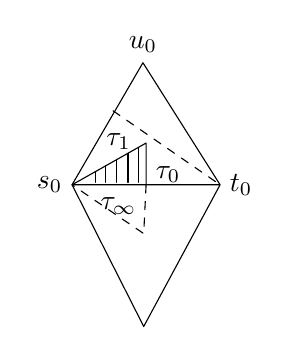
\begin{tikzpicture}[x=1cm,y=1cm,line cap=round,line join=round]
\draw (0,0)--(.9,1.55) node[above]{$u_0$} --(1.88,0) node[right]{$t_0$}--(.91,-1.8)--(0,0) node[left]{$s_0$}--(1.88,0);
\draw[dashed] (.52,.94)--(1.88,0);
\draw (0,0)--(.94,.53)--(.94,0);
\draw[dashed] (.94,0)--(.91,-.62)--(0,0);
\foreach \x in {.30,.43,.57,.71,.84}{\draw (\x,.03)--(\x,{.53*\x/.94});}
\node at (.59,.55){$\tau_1$};\node at (1.22,.13){$\tau_0$};\node at (.59,-.27){$\tau_\infty$};
\end{tikzpicture}}

% L20–22
La relation 22 s'écrit aussi, posant $g^{-1}a=u$
\[
\exists u\in U\quad\text{tel que}\quad\rho^{-1}(ua^{-1})a^{-1}\in\widetilde U\qquad\text{i.e.}\tag*{\deleted{(22)}}
\]
\[
\begin{aligned}
&\text{i.e. }\rho(a)a\in\unsure{\rho(\widetilde U).u|{\rho(\widetilde U).U}} \qquad
a\,\rho^{-1}(au^{-1})\in\widetilde U\quad\text{i.e. }a\,\rho^{-1}(a)\in\widetilde U\,\rho^{-1}(u),\\
&\hspace{9em}\deleted{\text{i.e. }\rho(a)a\in\rho(\widetilde U)U}
\end{aligned}
\]

% archive sheet number: 184
\scanpage{186}
% L01–02
ou encore
\[
\rho(a)\deleted{\unsure{\rho}}(a)\in\rho(\widetilde U)\deleted{\unsure{g^{-1}|\rho^{-1}}}.\deleted{\unsure{g}}\widetilde U\bigr)
\]

% L03–07
Posons $\widetilde U_0=\widetilde U=G_{0\,s_0}$, $\underset{\substack{\shortparallel\\\rho(\widetilde U)}}{\widetilde U_1}=G_{0\,t_0}$, la condition envisagée s'écrit donc
\[
\rho(a)\,a\in\widetilde U_1\widetilde U_0\tag*{(24)}
\]
(en plus de la relation
\[
a\in\operatorname{Norm}_{G_0}(\widetilde U_1)\bigr).
\]

% L08–14
\uline{NB} Dans le cas où le polyèdre $P_0$ est orienté, il est plus sympathique dans cette \unsure{traduction} de travailler dans $G_0^+$ (qui est encore transitif sur $S$ et $=$ sur l'ens. des arêtes orientées, qui est $=$ un \uline{torseur} sous $\unsure{G_\infty^+|G_0^+}$), en décrivant $a$ par un élément de $G_0^+$
\[
a\in\operatorname{Norm}_{G_0^+}(\overset{\deleted{\sim}}{U}_0)\qquad U_0=G^+_{0\,s_0}=\widetilde U_0\cap G_0^+ \tag*{(25)}
\]
et en écrivant \deleted{\unsure{(2|la}} alors (24) \inserted{dans $G_0^+$,} sous la forme équivalente
\[
\rho(a)a\in\overset{\deleted{\sim}}{U}_1.U_0\ .\tag*{(24')}
\]

% L15–20
On dit que l'homothétie \inserted{$\lambda$} est stricte si elle satisfait la condition que la structure de graphe \inserted{via} $A_\lambda\in\unsure{\mathfrak P_2(S)|\mathrm P_2(S)}$ définie par
\[
\deleted{\{s,t\}\in}\left\{\begin{aligned}
&A_\lambda=\bigl\{\{s,\lambda t\}\in\mathfrak P_2(S)\mid(s,t)\in S^2,\ \{s,t\}\in A_0\bigr\}\\
&\text{i.e. }\deleted{\{s,t\}\in\unsure{A}}\ \forall s,t\in A_0\qquad
\{s,t\}\in A_0\Longleftrightarrow\{s,\lambda t\}\in A_\lambda
\end{aligned}\right.\tag*{(25)}
\]
est isomorphe à $(S,A_{\unsure{0|\lambda}})$, \deleted{\illegible{1}} condition qu'on

% archive sheet number: 185
\scanpage{187}
\mspage{96}
% L01–03
peut aussi \deleted{formuler} \inserted{expliciter} en termes de théorie des groupes. Notons que l'on aura alors
% slanted
\margin{il faudra y revenir par la suite\ldots}
\[
\operatorname{Et}_{A_0}(s)=\operatorname{Et}_{A_\lambda}(\lambda s)\tag*{(26)}
\]

% L03 margin
% slanted
\margin{Cette relation est indépendante de la condition que l'homothétie soit stricte -- mais si elle est stricte, $A_\lambda$ étant associée à une structure de polyèdre, la combinatoire induite par $A_\lambda$ sur une étoile $\inserted{E}$ de $A_\lambda$, i.e. une structure $A_{E,\lambda}\subset\unsure{\mathfrak P_2(E)|\mathrm P_2(E)}$, est donc une structure de polygône -- ce qui ne semble peut être pas vrai autrement\ldots}

% L04–08
$s\in S$, donc les deux structures de graphe $A_0$ et $A_\lambda$ donnent lieu aux mêmes étoiles -- mais avec des centres différents : Le centre $\lambda s$ de l'étoile $E$, pour la structure $\Gamma_\lambda=\underset{2}{(}S,A_\lambda)$, est l'antipodique du centre $s$ pour $\Gamma_0$, via l'antipodisme $\lambda$.

% L09–19
Considérons alors le groupe $G_{0\,s}=G_{0\,(s'=\lambda.s)}$, \deleted{et le sous} le sous-groupe des rotations relatif à \deleted{\unsure{leur}} $s$ est le seul sous-groupe cyclique d'ordre $n$ de $G_{0\,s}\simeq\mathbb D_n$, donc est égal au sous-groupe correspondant \deleted{pour} relatif à $s'$, Cela montre que sur l'étoile $s$, les structures de polygône, induites par $A_0$ et $A_\lambda$ respectivement, ont $=$ groupe de rotations, i.e. sont transformées l'une de l'autre par un élément \inserted{$\gamma$} de $(\mathbb Z/n\mathbb Z)^*/\{\pm1\}=Z'_n$ ($n$ étant l'ordre des points de $S$) :
\[
\alpha_{E,\lambda}=(\alpha_{E,0})^{(\gamma)},\qquad\gamma\in Z'_n=(\mathbb Z/n\mathbb Z)^*/\pm1\tag*{(27)}
\]

% archive sheet number: 186
\scanpage{188}
% L01–04
L'\deleted{\unsure{entier}}\inserted{élément} $\gamma$ dépend a priori du choix de $s$, Mais \deleted{\unsure{si $s$|si on}} par transport de structure, on voit qu'il est le $=$ pour $s$ et \inserted{pour} $us$, $u\in G_0$, donc que il est en fait indépendant de $s$.

% L05–09
Mais \deleted{cela montre que l'on a} \inserted{on voit alors que} la structure $A_\lambda$ est entièrement déterminée par \deleted{\unsure{l'entier|l'indice}} l'élément
\[
\gamma\in Z'_n=(\mathbb Z/n\mathbb Z)^{\unsure{*|d}}/\pm1\tag*{(28)}
\]
puisque l'on a
\[
A_\lambda=\bigcup_{\substack{E\in{\unsure{\mathscr E|\mathcal E|\Sigma}}^{\unsure{a|0}}\\\text{ens des étoiles de } S\\(\text{le }=\text{ pour }A_0\text{ et }A_\lambda}}
\bigl(A_{E,\lambda}=A_{E,\unsure{0|.}}^{(\gamma)}\bigr).\tag*{(29)}
\]

% L10–16
Cet argument marche si, au lieu de supposer l'homothétie stricte, on suppose la chose suivante
\[
\deleted{\unsure{\mathrm P_2}}\left\{\begin{aligned}
\text{b)}\ &\text{Toute étoile }\inserted{E}\text{ est, }\deleted{\unsure{E}}\text{ pour la structure}\\
&A_{\lambda E}=A_\lambda\cap\unsure{\mathfrak P_2(E)|\mathrm P_2(E)},\ \text{un polygône}\\
&\text{combinatoire}\\
\text{a)}\ &\text{Toute }a\in A_\lambda\text{ est contenue dans}\\
&\text{au moins une étoile}
\end{aligned}\right.\tag*{(30)}
\]
% Curved transposition arrow from b) pointing below a).
\noindent\smash{\raisebox{1.3ex}{\begin{tikzpicture}[overlay]\draw[->] (0,1.4) to[bend right=30] (.26,0);\end{tikzpicture}}}

% L17–22
Notons que le groupe $G_0$ opère par automorphismes de $A_\lambda$, et qu'il opère transitivement sur l'ens des arêtes orientées de $G_0$. Il en résulte que \inserted{il suffit de vérifier} les conditions a) b) pour \uline{une} étoile $E$, pour \uline{une} arête $a$. \deleted{\unsure{de}} Pour la condition a) il suffit de prouver donc

% archive sheet number: 187
\scanpage{189}
\mspage{97}
% L01–08
qu'il existe au moins un ``triangle'' pour $A_\lambda$, i.e. \inserted{un triplet} des sommets \deleted{$\{s,t,u\}$} mutuellement adjacents pour $A_\lambda$. \deleted{\unsure{Il sera loisible}} OPS que ce triplet est \deleted{$\{s,\lambda t,u\}$ avec} de la forme
\[
\{s,\lambda t,u\}\qquad \text{avec }\{s,\lambda t\}\in A_\lambda\quad\text{i.e. }\{s,t\}\in A_0
\]
et il reste à \deleted{pour} vérifier l'existence d'un $u$ qui convient, i.e. tel que l'on ait
% L09–12
\[
\begin{aligned}
&\{s,u\}\ \&\ \{\lambda t,u\}\in A_\lambda\qquad\text{i.e.}\\
&\{\lambda^{-1}s,\deleted{\unsure{\lambda t}}u\},\{\unsure{t|\bar t},u\}\in A_0
\end{aligned}
\]
donc la condition b) signifie aussi
\[
\text{a$'$) Si }\{s,t\}\in A_0,\ \text{alors }\quad
\mathrm{Et}_{A_0}(t)\cap\mathrm{Et}_{A_0}(\lambda^{-1}s)\ne\varnothing \tag*{(31)}
\]
% L13–19
condition qu'il suffit de vérifier pour \uline{un} couple $(s,t)$ de sommets adjacents pour $A_0$. Cela s'énonce aussi \deleted{\unsure{(en adm. que $s$ est $t$)|(en \illegible{1} $s$ et $t$)}}
\[
\begin{aligned}
&\text{a$''$) }\deleted{\unsure{\forall\,s\in S,\ s|\forall s\in S}}\ \text{(Pour un }s\in S,\ \text{ou tout }s\in S,\ \text{c'est Kif-Kif)}\\
&\text{La distance combinatoire de }\lambda^{-1}s\text{ à }s\\
&\text{est }\leq 3\quad\text{(et en fait, égale à 3,}
\end{aligned}\tag*{(32)}
\]
% L20–23
sauf si $\lambda=\text{identité}$, \inserted{où elle est 0} ou dans le cas de l'octaèdre et $\lambda=$ \deleted{\unsure{antip.|antip}} \inserted{l'}antip. disons (où elle est $2$).
\diagram{\begin{tikzcd}[ampersand replacement=\&,column sep=small] \overset{s}{\bullet}\arrow[r,dash]\&\overset{t}{\bullet}\arrow[r,dash]\&\overset{t'}{\bullet}\arrow[r,dash]\&\overset{\lambda^{-1}s}{\bullet}\end{tikzcd}}
% L24–31
Si elle est égale à $0$ on a $\lambda^{-1}s=s$ i.e. $\lambda=id$ ; elle ne peut être égale à $1$ puisque \deleted{$s$ et $t$ (adjacents)} \inserted{deux sommets adj.} n'ont pas $=$ stabilisateur. Si elle était égale à $2$ i.e. \inserted{$\lambda\ne id$ et} $\exists\,t$ adjacent à 2 fois à $s$ et $\lambda^{-1}s$, on aurait $\mathrm{Et}_{A_0}(s)=\mathrm{Et}_{A_0}(\lambda^{-1}s)$ et $s\ne\lambda^{-1}s$, c'est le cas de l'octaèdre.

% archive sheet number: 188
